\documentclass[twocolumn]{extarticle}
\usepackage{fontspec}   %加這個就可以設定字體
\usepackage{xeCJK}       %讓中英文字體分開設置
\usepackage{indentfirst}
\usepackage{listings}
\usepackage[newfloat]{minted}
\usepackage{float}
\usepackage{graphicx}
\usepackage{caption}
\usepackage{fancyhdr}
\usepackage{hyperref}
\usepackage{amsmath}
\usepackage{multirow}
\usepackage[dvipsnames]{xcolor}
\usepackage{graphicx}
\usepackage{tabularx}
\usepackage{booktabs}
\usepackage{caption}
\usepackage{subcaption}
\usepackage{pifont}
\usepackage{amssymb}
\usepackage{titling}

\usepackage{pdftexcmds}
\usepackage{catchfile}
\usepackage{ifluatex}
\usepackage{ifplatform}

\usepackage[breakable, listings, skins, minted]{tcolorbox}
\usepackage{etoolbox}
\setminted{fontsize=\footnotesize}
\renewtcblisting{minted}{%
    listing engine=minted,
    minted language=python,
    listing only,
    breakable,
    enhanced,
    minted options = {
        linenos, 
        breaklines=true, 
        breakbefore=., 
        % fontsize=\footnotesize, 
        numbersep=2mm
    },
    overlay={%
        \begin{tcbclipinterior}
            \fill[gray!25] (frame.south west) rectangle ([xshift=4mm]frame.north west);
        \end{tcbclipinterior}
    }   
}

\usepackage[
top=1.5cm,
bottom=0.75cm,
left=1.5cm,
right=1.5cm,
includehead,includefoot,
heightrounded, % to avoid spurious underfull messages
]{geometry} 

\newenvironment{code}{\captionsetup{type=listing}}{}
\SetupFloatingEnvironment{listing}{name=Code}



\title{Deep Learning Lab 1 - Backpropagation}
\author{110550088 李杰穎}
\date{\today}


\setCJKmainfont{Noto Serif TC}


\ifwindows
\setmonofont[Mapping=tex-text]{Consolas}
\fi

\XeTeXlinebreaklocale "zh"             %這兩行一定要加,中文才能自動換行
\XeTeXlinebreakskip = 0pt plus 1pt     %這兩行一定要加,中文才能自動換行

\newcommand*{\dif}{\mathop{}\!\mathrm{d}}


\setlength{\parindent}{0em}
\setlength{\parskip}{2em}
\renewcommand{\baselinestretch}{1.25}
\setlength{\droptitle}{-7.5em}   % This is your set screw
\setlength{\columnsep}{2em}

\usepackage[moderate]{savetrees}

\begin{document}

\maketitle

\section{Introduction}
In this lab, I implement a simple multi-layer perceptron (MLP) with two hidden layers. Neural networks like MLPs form the foundation of many modern deep learning approaches and provide insights into how complex patterns can be learned from data. This implementation demonstrates the fundamental principles that underpin more sophisticated architectures used in contemporary deep learning systems.

The MLP architecture is applied to classify both linearly-separable data and the classical XOR problem. The XOR problem is particularly significant in the history of neural networks because it cannot be solved by a single-layer perceptron, making it a canonical test case for evaluating the representational power of neural networks with hidden layers. By successfully implementing backpropagation and training this network on the XOR problem, we demonstrate the essential capability of multi-layer architectures to learn complex non-linear relationships.

To develop a complete end-to-end learning system, I implement several core components: Mean Squared Error (MSE) loss function, a stochastic gradient descent optimizer, Sigmoid and ReLU activation functions, and the backpropagation algorithm for each component. This implementation provides hands-on experience with the fundamental building blocks that constitute modern deep learning frameworks and offers valuable insights into their inner workings.

\section{Implementation Details}
\subsection{Code structure}
The implementation is organized into modular components, with each functionality encapsulated in a separate file within the \texttt{src/} directory:
\begin{itemize}
\item \texttt{data.py}: Contains data generation utilities, including the provided \texttt{generate\_linear} and \texttt{generate\_XOR\_easy} functions.
\item \texttt{model.py}: Defines all architectural components required for constructing an MLP.
\item \texttt{loss.py}: Implements the MSE loss function.
\item \texttt{optimizer.py}: Implements the SGD optimizer.
\item \texttt{utils.py}: Contains visualization and plotting utilities.
\item \texttt{train.py}: Implements the main training loop and serves as the entry point for the implementation.
\end{itemize}

All neural network components inherit from an abstract \texttt{NNModule} parent class. This base class defines three essential methods that constitute the foundation of neural network operations:
\begin{enumerate}
\item \texttt{forward}: Implements the forward pass where inputs are propagated through the network to produce outputs. This method defines the computational behavior of each network component during inference.
\item \texttt{backward}: Handles the backward pass (gradient backpropagation), where gradients are computed with respect to parameters and inputs. This method enables the network to learn by calculating the gradients needed for parameter updates.
\item \texttt{parameters}: Provides access to the learnable parameters and their corresponding gradients that are necessary during optimization. This method allows the optimizer to efficiently update the network's parameters based on computed gradients.
\end{enumerate}

This design establishes a consistent interface for all neural network components, enabling modular design and seamless integration of different layers and functions within the network architecture—a pattern similar to that found in modern deep learning frameworks like PyTorch and TensorFlow.

\subsection{Sigmoid function}
The Sigmoid function is formally defined as:
\begin{equation}
\text{Sigmoid}(x) = \frac{1}{1+e^{-x}} \, .
\end{equation}
We derive its derivative with respect to its input $x$. Denoting $\text{Sigmoid}(x)$ as $\sigma(x)$:
\begin{align}
\frac{d}{dx} \sigma(x) &= \frac{d}{dx} \left[\frac{1}{1+e^{-x}}\right]  \\
&= \frac{e^{-x}}{(1+e^{-x})^2} \\
&= \frac{1}{1+e^{-x}} \frac{e^{-x}}{1+e^{-x}} \\
&= \sigma(x) \left(\frac{1+e^{-x}}{1+e^{-x}} - \frac{1}{1+e^{-x}}\right) \\
&= \sigma(x) \left(1 - \sigma(x)\right) \, .
\end{align}

A key observation is that the derivative of the Sigmoid function can be expressed solely in terms of its output $\sigma(x)$. This elegant property simplifies implementation and computational efficiency, as we can reuse the forward pass result when computing gradients.

\begin{code}
\captionof{listing}{\textbf{Implementation of the Sigmoid activation function.}}
\label{code: sigmoid}
\begin{minted}
class Sigmoid(NNModule):
    def __init__(self):
        self.output = None

    def forward(self, x):
        self.output = 1 / (1 + np.exp(-x))
        return self.output

    def backward(self, grad):
        return grad * self.output * (1 - self.output)

    def parameters(self):
        return []  # Activation functions don't have trainable parameters
\end{minted}
\end{code}

\subsection{Linear layer}

The linear layer is the fundamental building block of MLPs. It performs an affine transformation on the input data using weight matrix $W \in \mathbb{R}^{m \times n}$ and bias vector $b \in \mathbb{R}^m$, where $n$ and $m$ represent the number of input and output features, respectively. Formally, the linear transformation is defined as:

\begin{equation}
\text{Linear}(x) = xW^T + b \,.
\end{equation}

The weight matrix $W$ is defined with dimensions $m \times n$ to facilitate more efficient matrix operations during both forward and backward passes, particularly when implementing backpropagation.

\begin{code}
\captionof{listing}{\textbf{Implementation of the Linear layer.}}
\label{code: linear}
\begin{minted}
class Linear(NNModule):
    def __init__(self, in_features, out_features, bias=True):
        self.in_features = in_features
        self.out_features = out_features

        # Convert weights and biases to Parameter objects
        self.weight = Parameter(np.random.randn(out_features, in_features))
        self.bias = Parameter(np.random.randn(out_features)) if bias else None

    def forward(self, x):
        self.x = x
        if self.bias is not None:
            return np.dot(x, self.weight.data.T) + self.bias.data
        return np.dot(x, self.weight.data.T)
\end{minted}
\end{code}

\subsection{Neural network architecture}
For this implementation, I designed a simple MLP with two hidden layers, each containing 16 neurons. The input layer has 2 neurons, corresponding to the x and y coordinates of the data points. The output layer consists of a single neuron that outputs the probability of an input coordinate belonging to the positive class. Bias terms are included in each layer to increase the model's expressivity.

For activation functions, ReLU is applied after the first hidden layer to introduce non-linearity, while Sigmoid is used after the second hidden layer to constrain the output to the [0,1] range, representing a probability value.

The complete MLP architecture is illustrated in Figure \ref{fig:mlp}.

\begin{figure}[H]
\centering
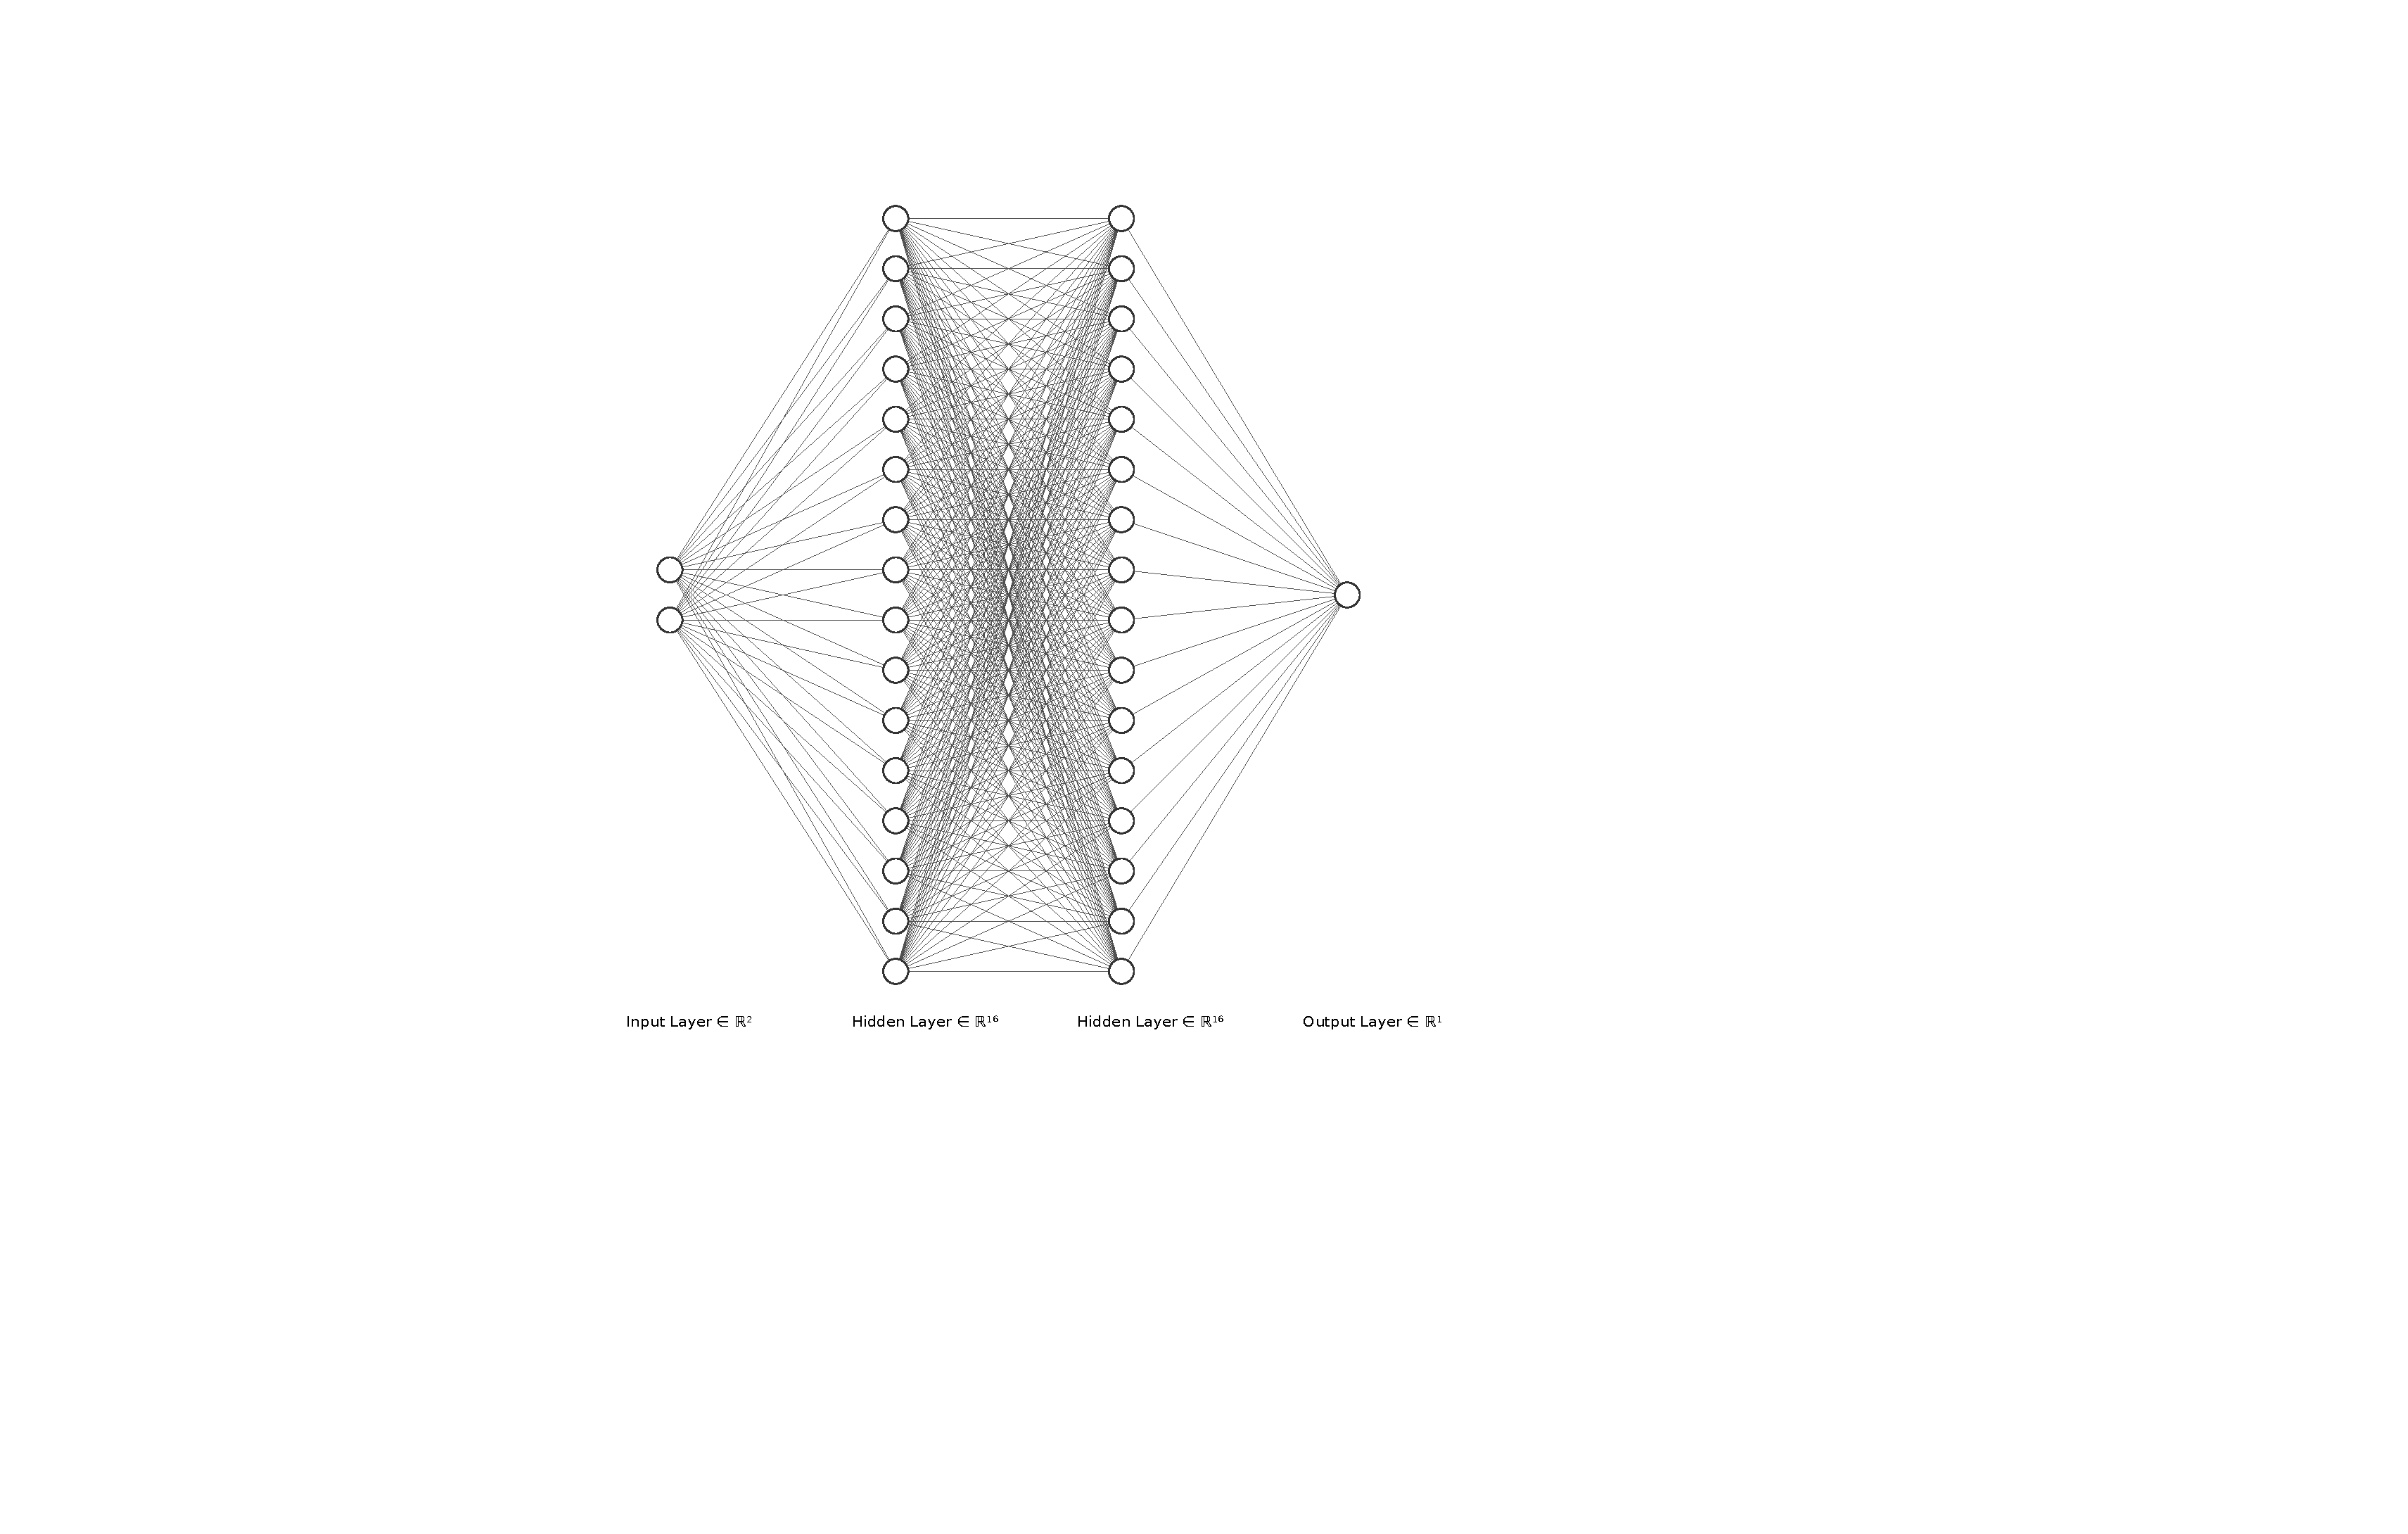
\includegraphics[width=0.95\linewidth]{figures/mlp}
\caption{\textbf{The MLP architecture with two hidden layers.} The network processes 2D input through two hidden layers with 16 neurons each, using ReLU and Sigmoid activations, culminating in a single output neuron for binary classification.}
\label{fig:mlp}
\end{figure}

Given the components described above, we can now construct the complete MLP and define its forward propagation mechanism.

\begin{code}
\captionof{listing}{\textbf{Implementation of the MLP architecture.}}
\label{code: mlp}
\begin{minted}
class MLP(NNModule):
    def __init__(self, in_features, hidden_size, out_features, activations=[ReLU(), Sigmoid()]):
        self.linear1 = Linear(in_features, hidden_size)
        self.linear2 = Linear(hidden_size, out_features)
        self.activation1, self.activation2 = activations

    def forward(self, x):
        x = self.linear1.forward(x)
        x = self.activation1.forward(x)
        x = self.linear2.forward(x)
        x = self.activation2.forward(x)
        return x

    def backward(self, grad):
        grad = self.activation2.backward(grad)
        grad = self.linear2.backward(grad)
        grad = self.activation1.backward(grad)
        grad = self.linear1.backward(grad)
        return grad

    def parameters(self):
        params = []
        params.extend(self.linear1.parameters())
        params.extend(self.linear2.parameters())
        return params
\end{minted}
\end{code}

\subsection{Backpropagation}

The backpropagation algorithm is implemented through the \texttt{backward} method in each module, which computes gradients for all parameters and returns the gradient with respect to the input. These gradients are stored in the \texttt{.grad} attribute of each parameter, making them accessible to the optimizer for parameter updates.

The design of the \texttt{Parameter} class is central to this implementation. Each \texttt{Parameter} object contains two attributes: \texttt{data}, which stores the actual parameter values (e.g., weights), and \texttt{grad}, which stores the computed gradients. This separation facilitates the optimization process by providing a clear interface for updating parameters based on their gradients.

While the \texttt{backward} methods for activation functions were derived earlier, let us focus on deriving the backward pass for the \texttt{Linear} layer.

For a linear layer with forward propagation defined as:
\begin{equation}
y = x W^T + b \, ,
\end{equation}
where $y\in\mathbb{R}^n$ is the output, $x\in \mathbb{R}^m$ is the input, $W \in \mathbb{R}^{n \times m}$ is the weight matrix, and $b \in \mathbb{R}^n$ is the bias vector, we need to compute the partial derivatives of the loss $L$ with respect to $W$, $b$, and input $x$:

\begin{align}
\frac{\partial L}{\partial W} &= \frac{\partial L}{\partial y} \frac{\partial y}{\partial W} =  \left(\frac{\partial L}{\partial y}\right)^T x \\
\frac{\partial L}{\partial b} &= \frac{\partial L}{\partial y} \frac{\partial y}{\partial b} = \sum_i \left(\frac{\partial L}{\partial y}\right)_i \\
\frac{\partial L}{\partial x} &= \frac{\partial L}{\partial y} \frac{\partial y}{\partial x} = \frac{\partial L}{\partial y} W \\
\end{align}

The backward method of the MLP orchestrates the entire backpropagation process by calling the backward methods of its components in reverse order, effectively implementing the chain rule of calculus for gradient propagation through the network.

\subsection{Optimizer and Training Loop}

The optimizer implements the parameter update strategy based on computed gradients. For this implementation, I use a simple Stochastic Gradient Descent (SGD) optimizer, which updates parameters in the direction of the negative gradient scaled by the learning rate:

\begin{code}
\captionof{listing}{\textbf{Implementation of the SGD optimizer.}}
\label{code:optimizer}
\begin{minted}
class Optimizer:
    def __init__(self, parameters, lr=0.01):
        self.parameters = parameters
        self.lr = lr

    def step(self):
        for param in self.parameters:
            param.data -= self.lr * param.grad
            param.grad = np.zeros_like(param.grad)

    def zero_grad(self):
        for param in self.parameters:
            param.grad = np.zeros_like(param.grad)


class SGD(Optimizer):
    def __init__(self, parameters, lr=0.01):
        super(SGD, self).__init__(parameters, lr)

    def step(self):
        for param in self.parameters:
            param.data -= self.lr * param.grad
            param.grad = np.zeros_like(param.grad)
\end{minted}
\end{code}

The optimizer provides two key methods:
\begin{enumerate}
    \item \texttt{zero\_grad()}: Resets all parameter gradients to zero before computing new gradients for the current iteration.
    \item \texttt{step()}: Updates all parameters by subtracting the gradient scaled by the learning rate.
\end{enumerate}

The training process is coordinated by the training loop, which orchestrates the forward pass, loss computation, backpropagation, and parameter updates for each training iteration:

\begin{code}
\captionof{listing}{\textbf{Implementation of the training loop.}}
\label{code:train}
\begin{minted}
def train(model, loss_fn, optimizer, x, y, epochs=1000):
    losses = []
    start_time = time.time()
    for epoch in range(epochs):
        optimizer.zero_grad()
        output = model.forward(x)
        loss = loss_fn.forward(output, y)
        grad = loss_fn.backward()
        model.backward(grad)
        optimizer.step()
        losses.append(loss)
        if epoch % 100 == 0:
            print(f'Epoch {epoch}, Loss {loss}')
    print(f'Epoch {epochs}, Loss {loss}')
    print(f'Training finished, elapsed {time.time() - start_time}s')
    # show loss
    if args.output_path:
        plot_loss(
            losses, args, f'{args.output_path}/loss_{args.data}_lr{str(args.lr).replace(".", "")}_n{args.num_neurons}_e{args.epochs}{"_no_acti" if args.no_activation else ""}.png')
    else:
        plot_loss(losses, args)
\end{minted}
\end{code}

Each training iteration follows this sequence:
\begin{enumerate}
    \item \textbf{Gradient reset}: The optimizer's \texttt{zero\_grad()} method clears any existing gradients.
    \item \textbf{Forward pass}: The model processes the input data and generates predictions.
    \item \textbf{Loss calculation}: The loss function computes the error between predictions and targets.
    \item \textbf{Backward pass}: The loss function initiates backpropagation by computing the initial gradient, which is then propagated backward through the model to compute gradients for all parameters.
    \item \textbf{Parameter update}: The optimizer updates all parameters based on their gradients.
    \item \textbf{Progress tracking}: The loss is recorded for later visualization, and periodic updates are printed to monitor training progress.
\end{enumerate}

At the conclusion of training, the cumulative loss history is visualized to provide insight into the training dynamics and convergence behavior.


\section{Experimental Results}
I conducted experiments on two datasets: linearly separable data and the XOR problem. For each experiment, the MLP was trained using the following hyperparameters:
\begin{itemize}
    \item Learning rate: 1.0
    \item Number of epochs: 100,000
    \item Number of neurons per hidden layer: 16
    \item Weight initialization: Normal distribution $\mathcal{N}(0, 1)$
\end{itemize}

\subsection{Linearly Separable Data}
For the linearly separable dataset, the model converged rapidly to an accurate decision boundary. Figure \ref{fig:linear_loss} illustrates the training loss curve, showing consistent and stable convergence, while Figure \ref{fig:linear_results} displays the final decision boundary learned by the model.

\begin{figure}[H]
\centering
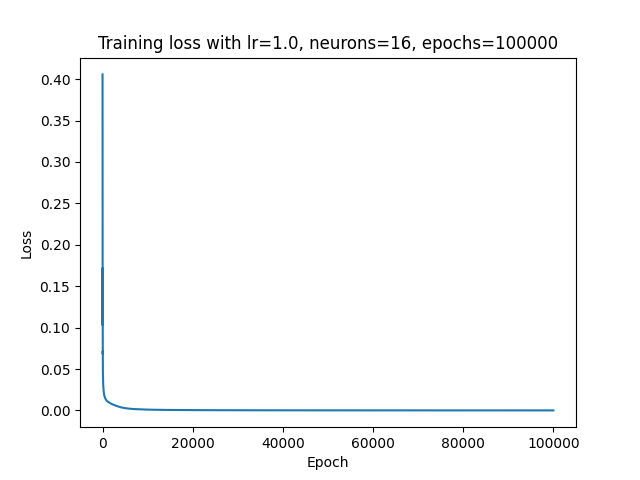
\includegraphics[width=0.95\linewidth]{figures/results/loss_linear_lr1_n16}
\caption{\textbf{Training loss curve for linearly separable data.} The loss decreases smoothly and monotonically, indicating stable convergence without oscillation.}
\label{fig:linear_loss}
\end{figure}

\begin{figure}[H]
\centering
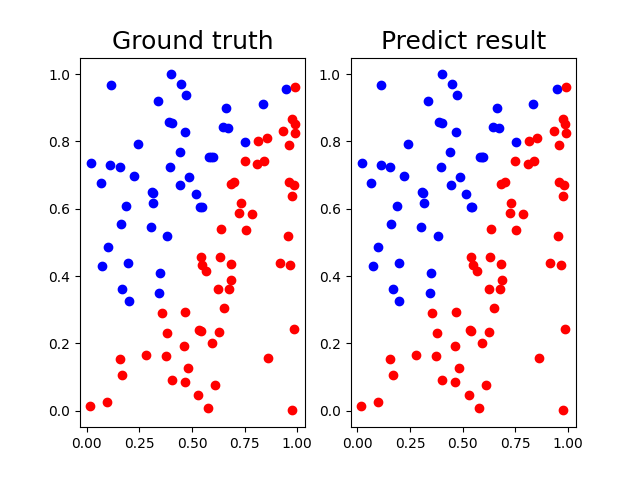
\includegraphics[width=0.95\linewidth]{figures/results/linear_lr1_n16}
\caption{\textbf{Decision boundary learned by the MLP on linearly separable data.} The network achieves perfect classification with 100\% accuracy (100/100 samples).}
\label{fig:linear_results}
\end{figure}

The model achieved 100\% accuracy on the linearly separable dataset. This result aligns with expectations, as even a simple network architecture can effectively learn the appropriate linear decision boundary.

\begin{figure}[H]
\centering
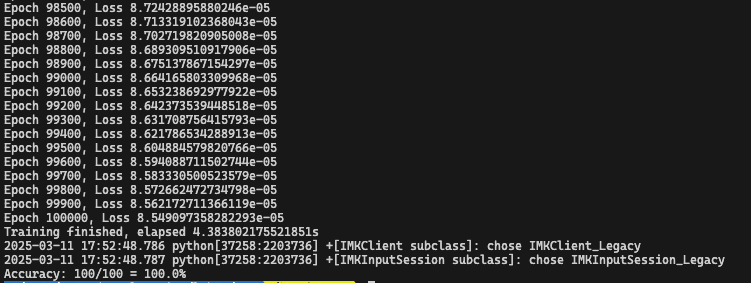
\includegraphics[width=0.95\linewidth]{figures/linear_loss_acc}
\caption{\textbf{The training loss and testing accuracy of linearly separable data.}}
\label{fig:linearlossacc}
\end{figure}


\subsection{XOR Problem}
The XOR problem presents a more challenging task as it requires a non-linear decision boundary. Figure \ref{fig:xor_loss} shows the training loss over epochs, while Figure \ref{fig:xor_results} illustrates the final decision boundary learned by the model.

\begin{figure}[H]
\centering
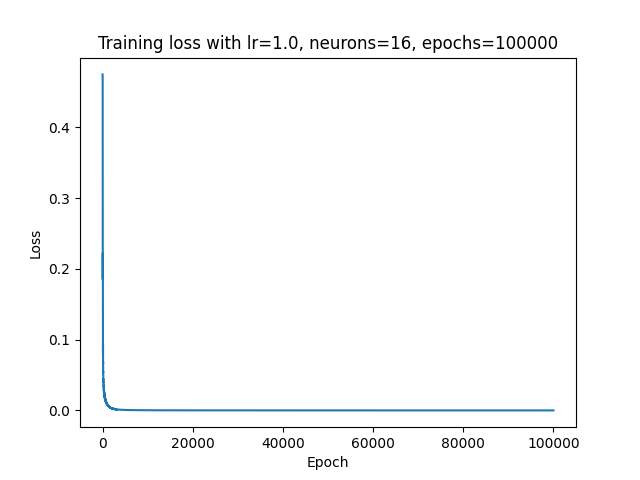
\includegraphics[width=\linewidth]{figures/results/loss_xor_lr1_n16}
\caption{\textbf{Training loss curve for the XOR problem.} The loss exhibits more complex dynamics compared to the linear problem but ultimately converges to a low value.}
\label{fig:xor_loss}
\end{figure}

\begin{figure}[H]
\centering
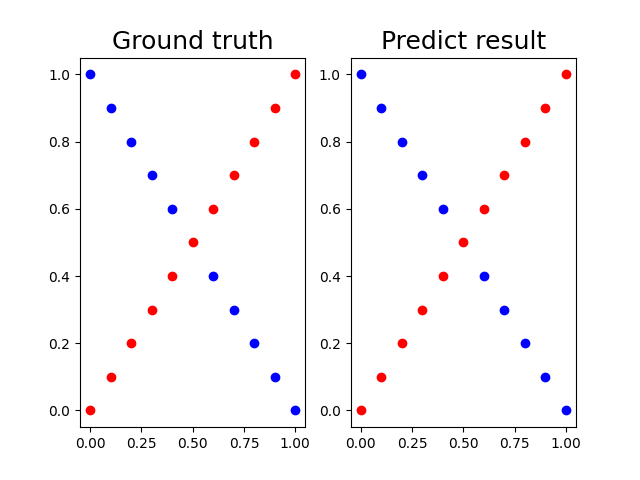
\includegraphics[width=0.95\linewidth]{figures/results/xor_lr01_n16}
\caption{\textbf{Decision boundary learned by the MLP on the XOR problem.} The network successfully forms a non-linear decision boundary that perfectly separates the classes with 100\% accuracy (21/21 samples).}
\label{fig:xor_results}
\end{figure}

For the XOR problem, the model achieved 100\% accuracy on the test set. The learned decision boundary clearly demonstrates how the model successfully captured the non-linear relationship, separating the two classes with a complex boundary. This result validates the theoretical capability of multi-layer networks with non-linear activation functions to solve problems beyond the limitations of linear models.

\begin{figure}[H]
\centering
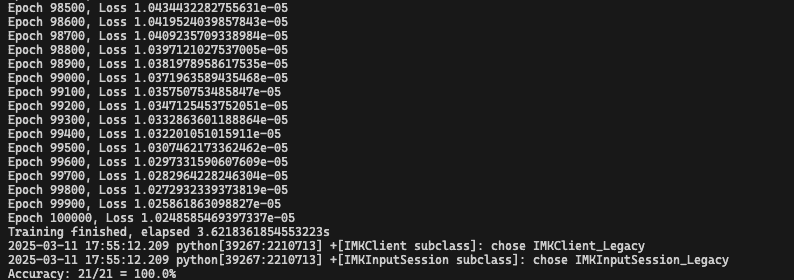
\includegraphics[width=0.95\linewidth]{figures/xor_loss_acc}
\caption{\textbf{The training loss and testing accuracy of XOR problem.}}
\label{fig:xorlossacc}
\end{figure}


\section{Discussion}

\subsection{Learning Rate Analysis}
We conducted experiments with four different learning rates and evaluated their performance over 500 training epochs. As shown in Figures \ref{fig:loss_linear} and \ref{fig:loss_xor}, the learning rate significantly impacts the convergence behavior and final performance of the network.

When the learning rate is set too high (e.g., 10), the loss function exhibits significant oscillation. Although the model eventually converges with a high learning rate, its final performance is suboptimal due to the inability to settle precisely at the minimum of the loss landscape. Conversely, with an excessively small learning rate (e.g., 0.01), the MLP fails to converge within the constraint of 500 epochs, as the parameter updates are too small to make sufficient progress toward the optimal solution.

Our experiments demonstrate that a learning rate of 1 yields optimal accuracy for both datasets, striking a balance between convergence speed and stability. This is quantified in Table \ref{tab:lr}, which shows the clear performance advantage of the moderate learning rate setting.

\begin{figure}[H]
\resizebox{0.95\linewidth}{!}{%
\begin{tabular}{cc}
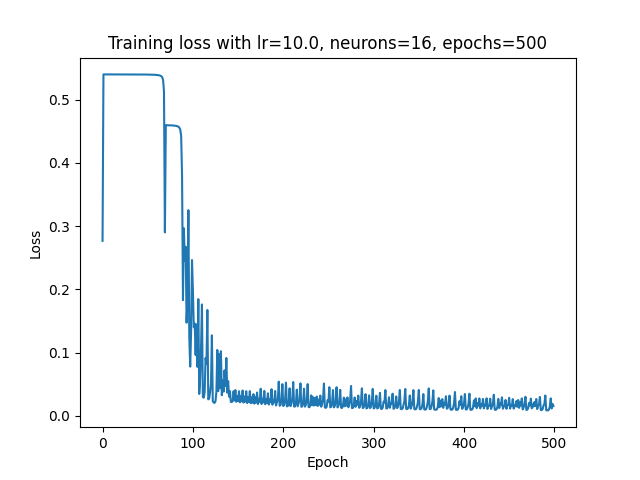
\includegraphics{figures/results/loss_linear_lr100_n16_e500} & 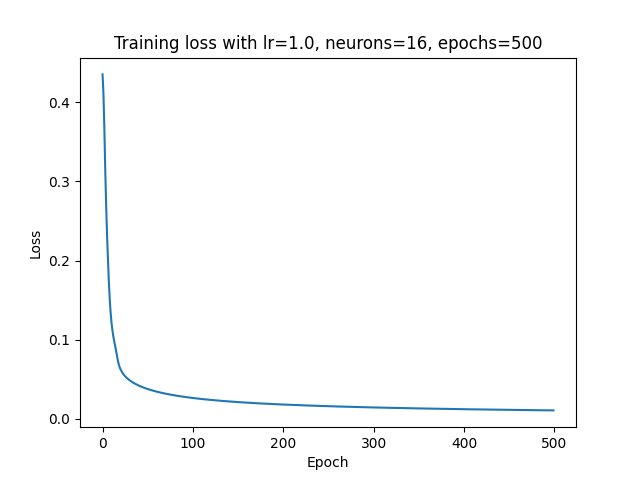
\includegraphics{figures/results/loss_linear_lr10_n16_e500} \\
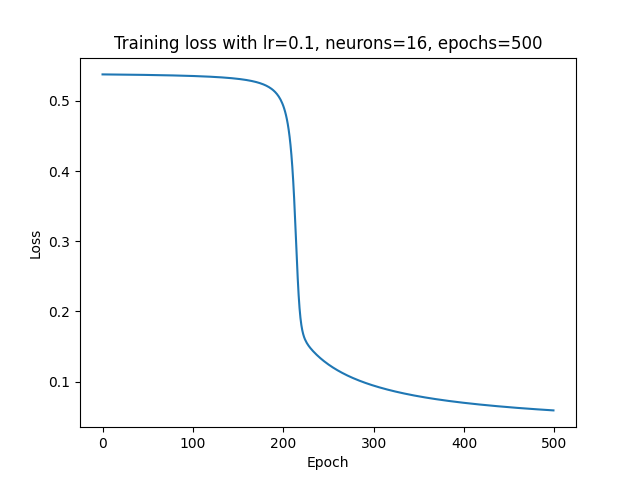
\includegraphics{figures/results/loss_linear_lr01_n16_e500} &
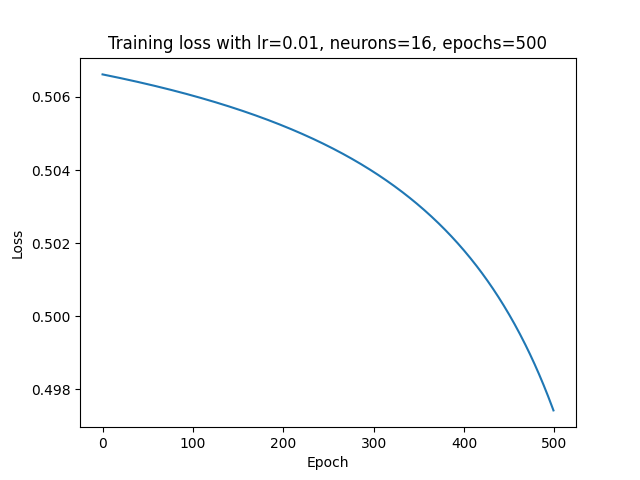
\includegraphics{figures/results/loss_linear_lr001_n16_e500}
\end{tabular}%
}
\caption{\textbf{Loss trajectories for linear classification with varying learning rates.} From top-left to bottom-right: lr=10, lr=1, lr=0.1, and lr=0.01. Note the oscillatory behavior with high learning rates and slow convergence with low learning rates.}
\label{fig:loss_linear}
\end{figure}

\begin{figure}[H]
\resizebox{0.95\linewidth}{!}{%
\begin{tabular}{cc}
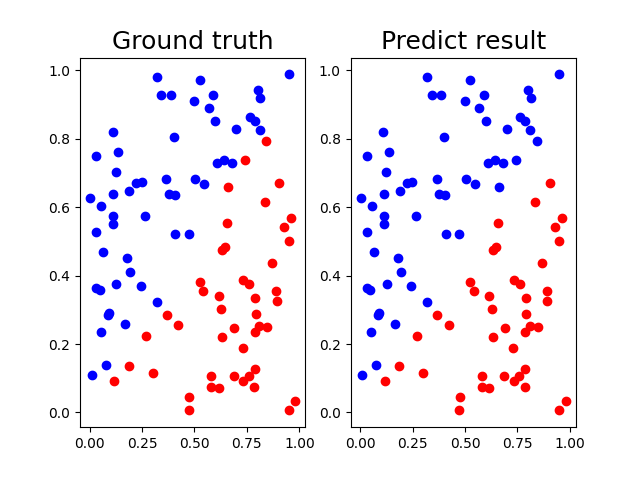
\includegraphics{figures/results/linear_lr100_n16_e500} & 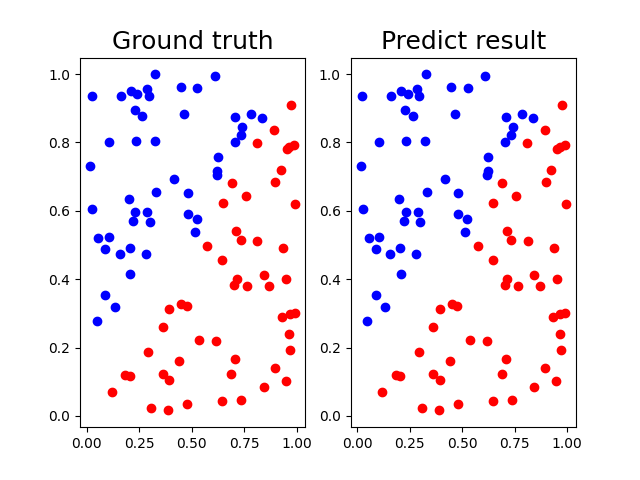
\includegraphics{figures/results/linear_lr10_n16_e500} \\
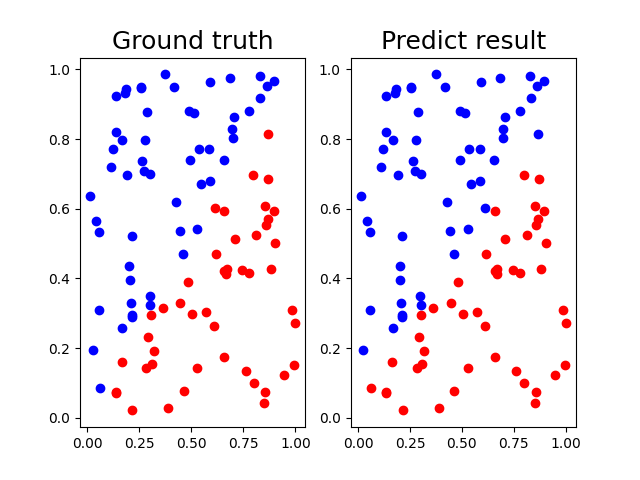
\includegraphics{figures/results/linear_lr01_n16_e500} &
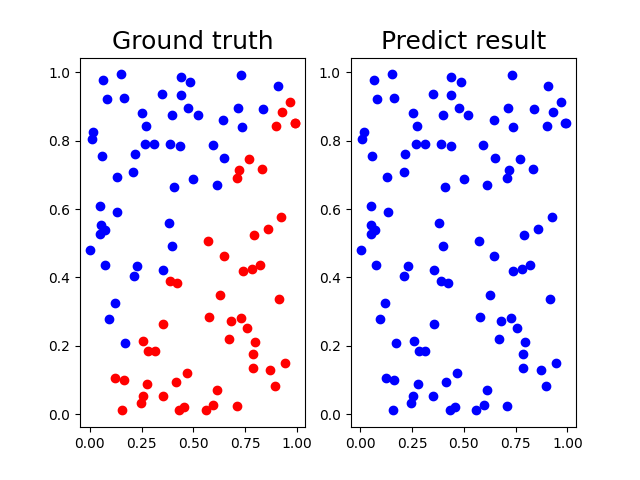
\includegraphics{figures/results/linear_lr001_n16_e500}
\end{tabular}%
}
\caption{\textbf{Decision boundaries for linear classification with varying learning rates.} From top-left to bottom-right: lr=10, lr=1, lr=0.1, and lr=0.01. The optimal learning rate (lr=1) produces the cleanest and most accurate decision boundary.}
\label{fig:res_linear}
\end{figure}

\begin{figure}[H]
\resizebox{0.95\linewidth}{!}{%
\begin{tabular}{cc}
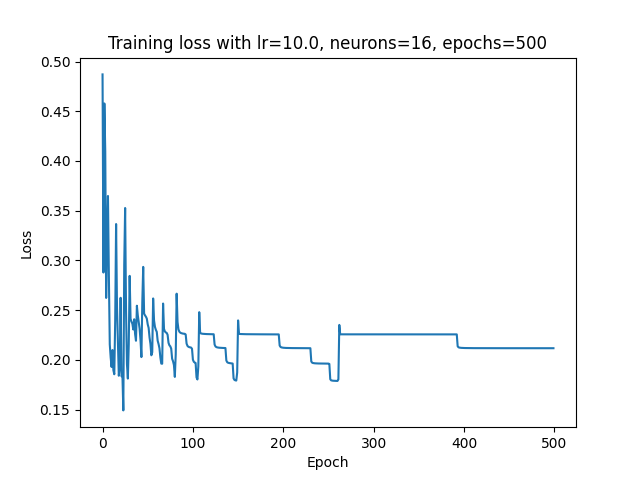
\includegraphics{figures/results/loss_xor_lr100_n16_e500} & 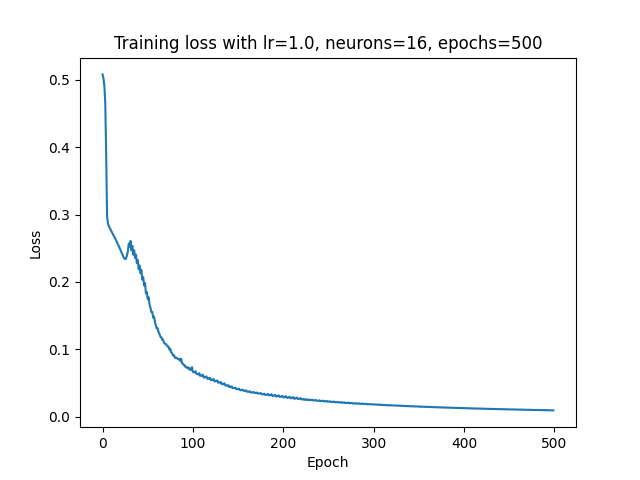
\includegraphics{figures/results/loss_xor_lr10_n16_e500} \\
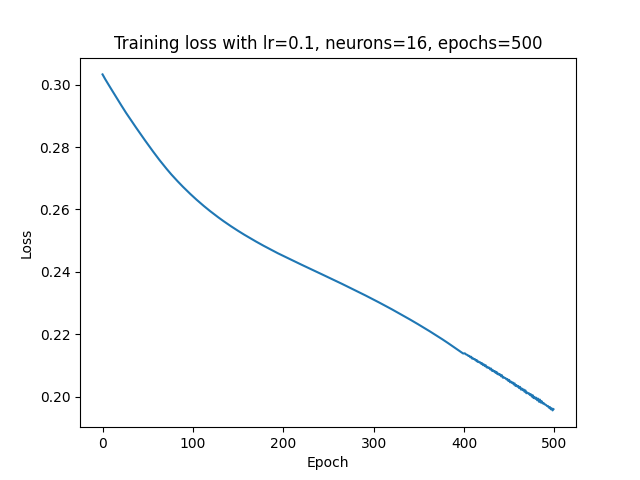
\includegraphics{figures/results/loss_xor_lr01_n16_e500} &
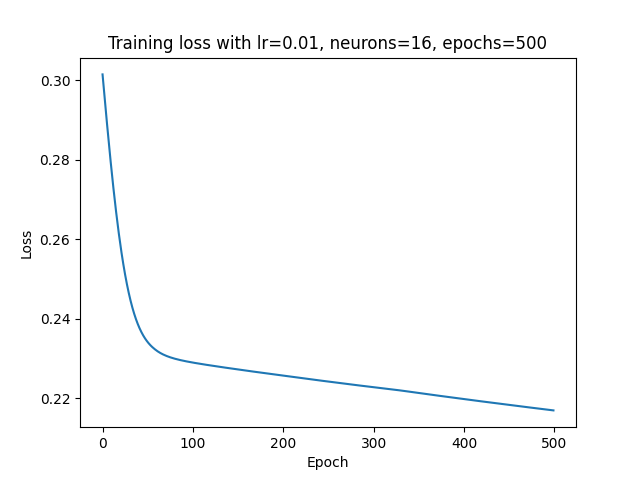
\includegraphics{figures/results/loss_xor_lr001_n16_e500}
\end{tabular}%
}
\caption{\textbf{Loss trajectories for XOR classification with varying learning rates.} From top-left to bottom-right: lr=10, lr=1, lr=0.1, and lr=0.01. The non-linear XOR problem exhibits more pronounced convergence differences across learning rates, with greater sensitivity to the choice of learning rate.}
\label{fig:loss_xor}
\end{figure}

\begin{figure}[H]
\resizebox{0.95\linewidth}{!}{%
\begin{tabular}{cc}
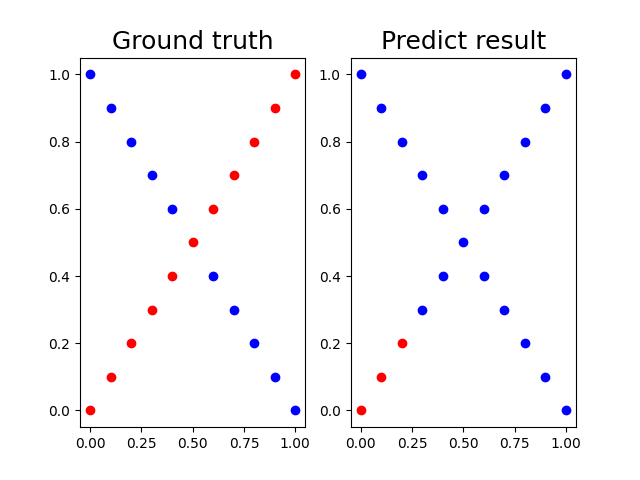
\includegraphics{figures/results/xor_lr100_n16_e500} & 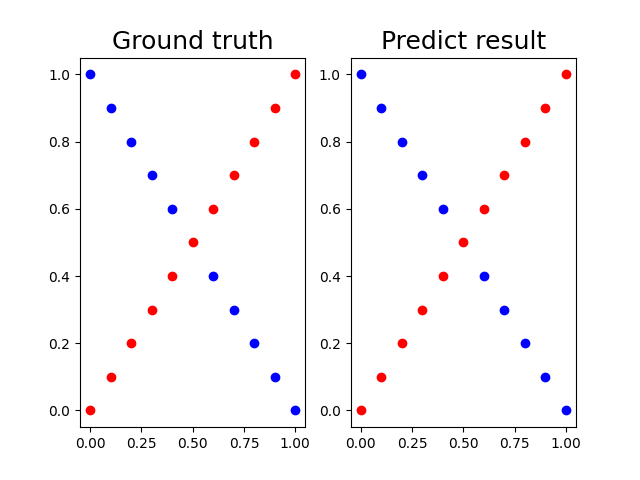
\includegraphics{figures/results/xor_lr10_n16_e500} \\
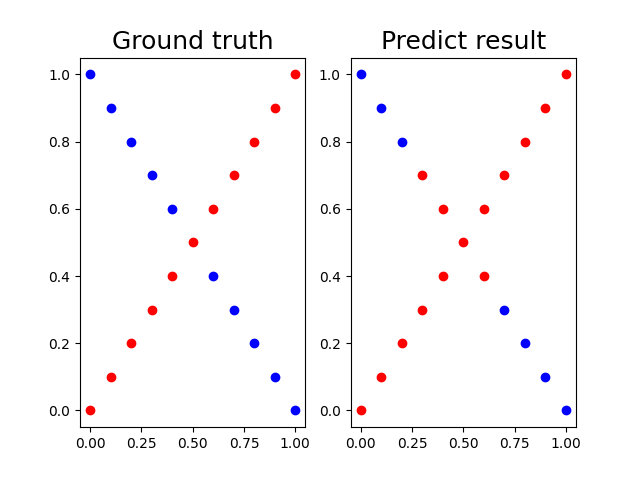
\includegraphics{figures/results/xor_lr01_n16_e500} &
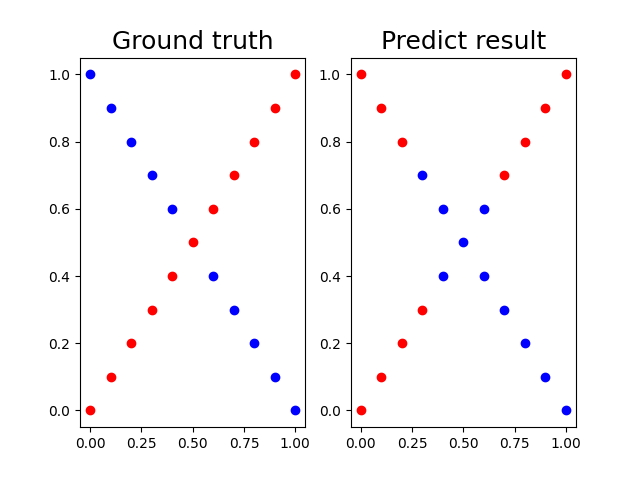
\includegraphics{figures/results/xor_lr001_n16_e500}
\end{tabular}%
}
\caption{\textbf{Decision boundaries for XOR classification with varying learning rates.} From top-left to bottom-right: lr=10, lr=1, lr=0.1, and lr=0.01. The complex non-linear decision boundary for the XOR problem requires a well-calibrated learning rate for optimal formation.}
\label{fig:res_xor}
\end{figure}

\begin{table}[t]
\centering
\caption{\textbf{Classification accuracy (\%) with different learning rates on linear and XOR datasets.} A learning rate of 1 achieves optimal performance on both tasks, while extremely high (10) or low (0.01) learning rates significantly degrade performance.}
\label{tab:lr}
\begin{tabular}{@{}ccc@{}}
\toprule
\textbf{Learning Rate} & \textbf{Linear} & \textbf{XOR} \\ \midrule
10          & 97.0            & 61.9         \\
1           & 100.0           & 100.0        \\
0.1         & 97.0            & 85.7         \\
0.01        & 49.0            & 42.9         \\ \bottomrule
\end{tabular}
\end{table}

\subsection{Number of Neurons Analysis}
We conducted experiments with four different network capacities by varying the number of neurons in the hidden layers and evaluated their performance over 500 training epochs. As shown in Figures \ref{fig:loss_linear_n} and \ref{fig:loss_xor_n}, the network architecture significantly impacts convergence behavior and representation capabilities.

With fewer neurons (e.g., 4), the network may lack sufficient capacity to capture complex patterns, particularly for the XOR dataset which requires non-linear decision boundaries. As we increase the number of neurons, the model's representational capacity improves, enabling it to learn more intricate decision boundaries with greater precision.

Our experiments demonstrate that while the linearly separable dataset can be effectively learned with as few as 4 neurons, the XOR problem requires at least 16 neurons to achieve optimal performance, as quantified in Table \ref{tab:num}. This result aligns with theoretical expectations regarding the minimum complexity required to represent certain functions, highlighting the relationship between model capacity and task complexity.

\begin{figure}[H]
\resizebox{0.95\linewidth}{!}{%
\begin{tabular}{cc}
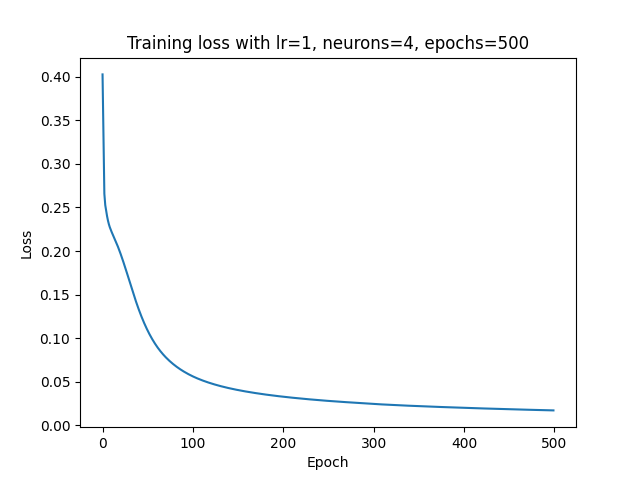
\includegraphics{figures/results/loss_linear_lr1_n4_e500} & 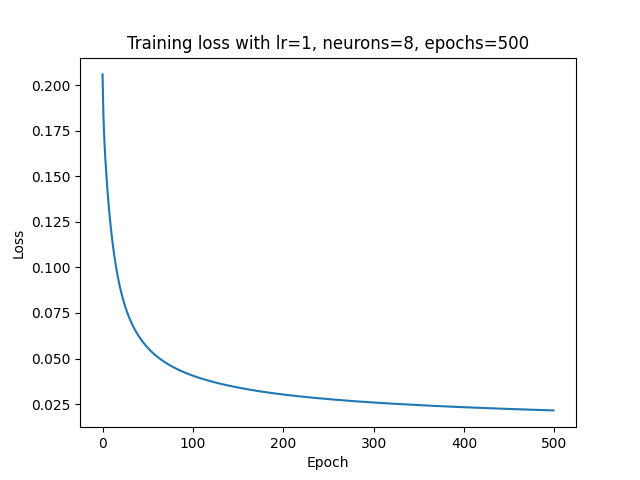
\includegraphics{figures/results/loss_linear_lr1_n8_e500} \\
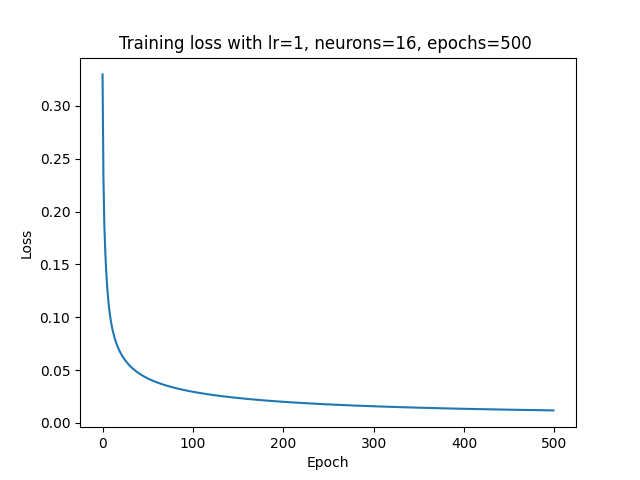
\includegraphics{figures/results/loss_linear_lr1_n16_e500} &
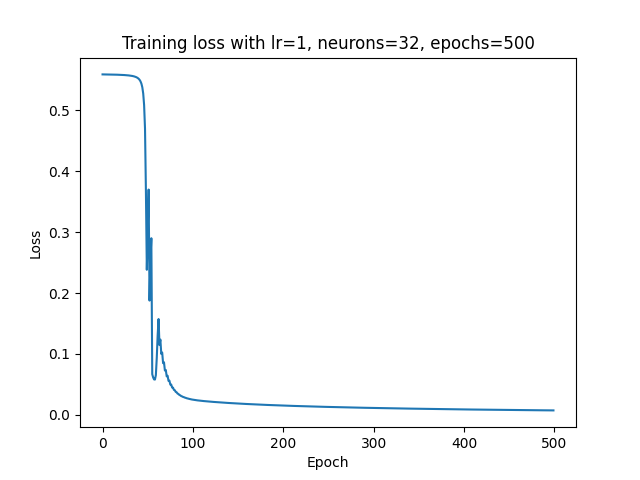
\includegraphics{figures/results/loss_linear_lr1_n32_e500}
\end{tabular}%
}
\caption{\textbf{Loss trajectories for linear classification with varying numbers of neurons.} From top-left to bottom-right: n=4, n=8, n=16, and n=32. The convergence patterns show subtle differences across different network capacities, with all configurations eventually reaching low loss values.}
\label{fig:loss_linear_n}
\end{figure}

\begin{figure}[H]
\resizebox{0.95\linewidth}{!}{%
\begin{tabular}{cc}
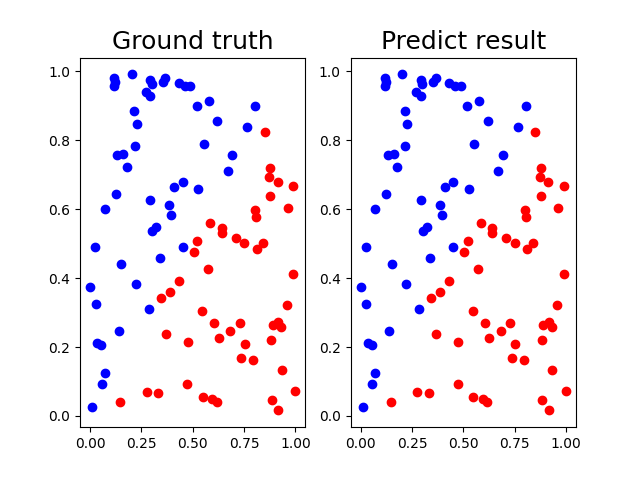
\includegraphics{figures/results/linear_lr1_n4_e500} & 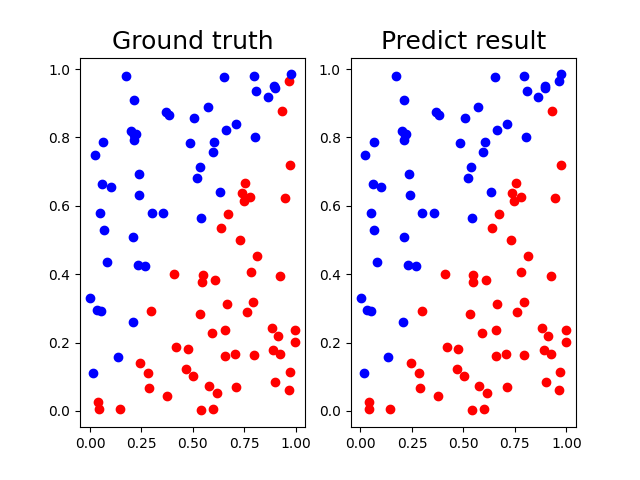
\includegraphics{figures/results/linear_lr1_n8_e500} \\
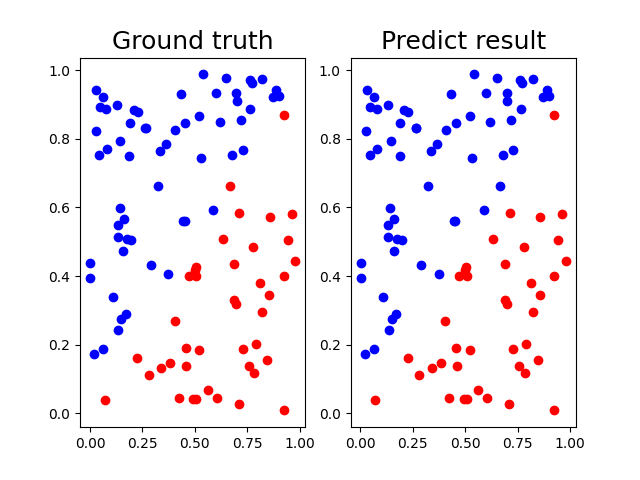
\includegraphics{figures/results/linear_lr1_n16_e500} &
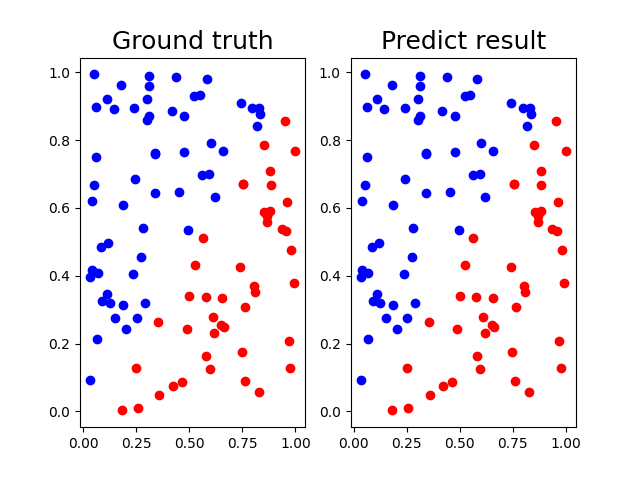
\includegraphics{figures/results/linear_lr1_n32_e500}
\end{tabular}%
}
\caption{\textbf{Decision boundaries for linear classification with varying numbers of neurons.} From top-left to bottom-right: n=4, n=8, n=16, and n=32. Even with minimal capacity, the network effectively learns appropriate linear decision boundaries for this task.}
\label{fig:res_linear_n}
\end{figure}

\begin{figure}[H]
\resizebox{0.95\linewidth}{!}{%
\begin{tabular}{cc}
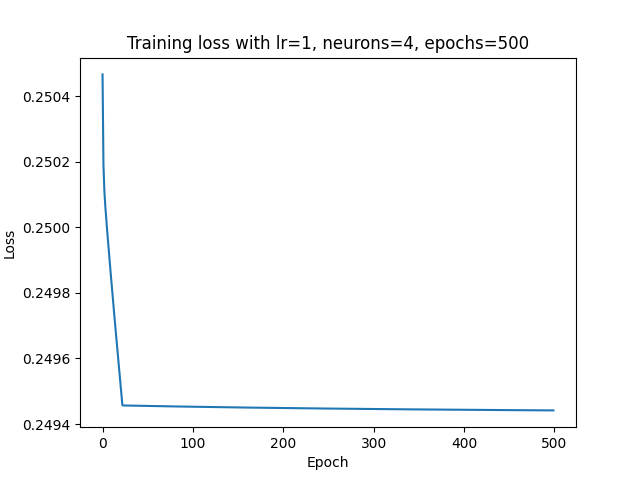
\includegraphics{figures/results/loss_xor_lr1_n4_e500} & 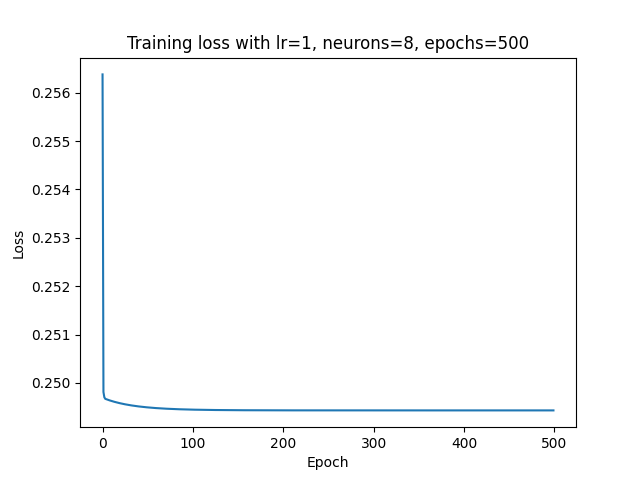
\includegraphics{figures/results/loss_xor_lr1_n8_e500} \\
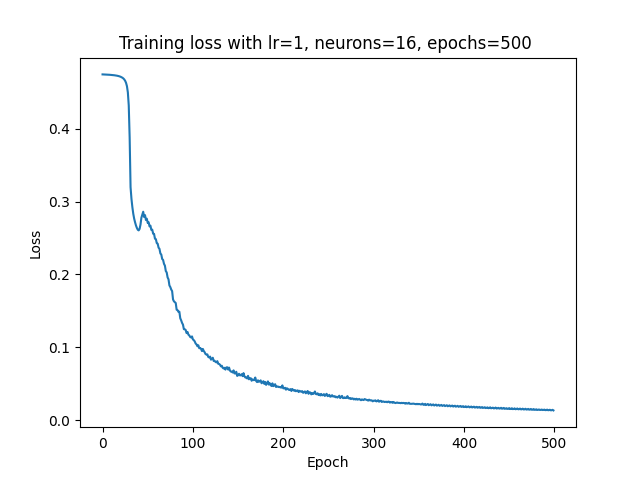
\includegraphics{figures/results/loss_xor_lr1_n16_e500} &
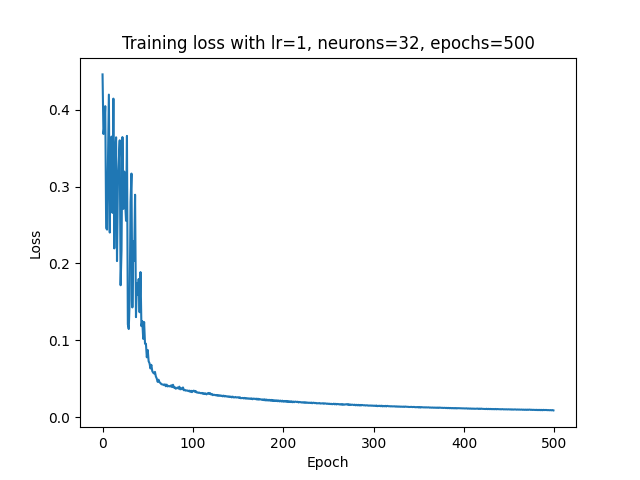
\includegraphics{figures/results/loss_xor_lr1_n32_e500}
\end{tabular}%
}
\caption{\textbf{Loss trajectories for XOR classification with varying numbers of neurons.} From top-left to bottom-right: n=4, n=8, n=16, and n=32. Networks with fewer neurons struggle to converge for this non-linear problem, demonstrating the relationship between model capacity and representational power.}
\label{fig:loss_xor_n}
\end{figure}

\begin{figure}[H]
\resizebox{0.95\linewidth}{!}{%
\begin{tabular}{cc}
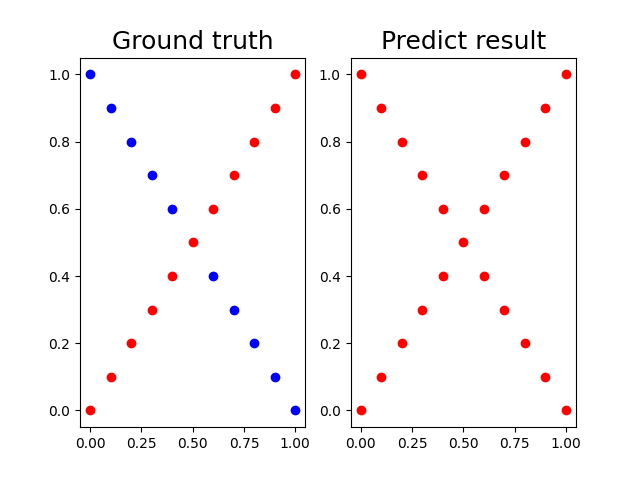
\includegraphics{figures/results/xor_lr1_n4_e500} & 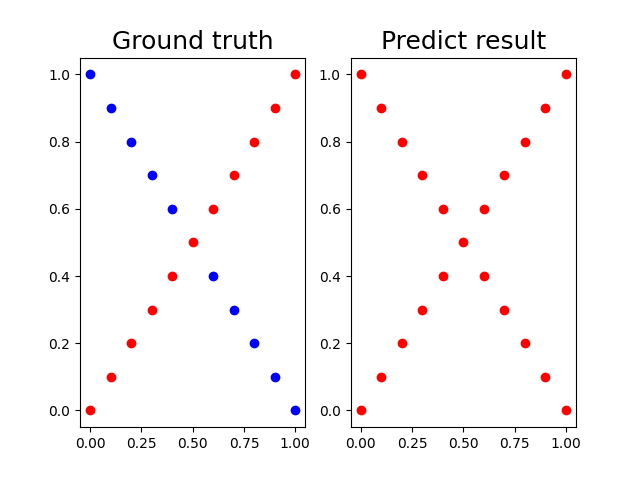
\includegraphics{figures/results/xor_lr1_n8_e500} \\
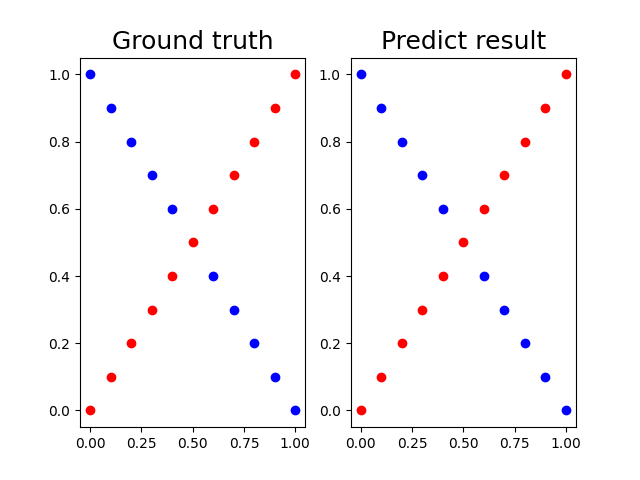
\includegraphics{figures/results/xor_lr1_n16_e500} &
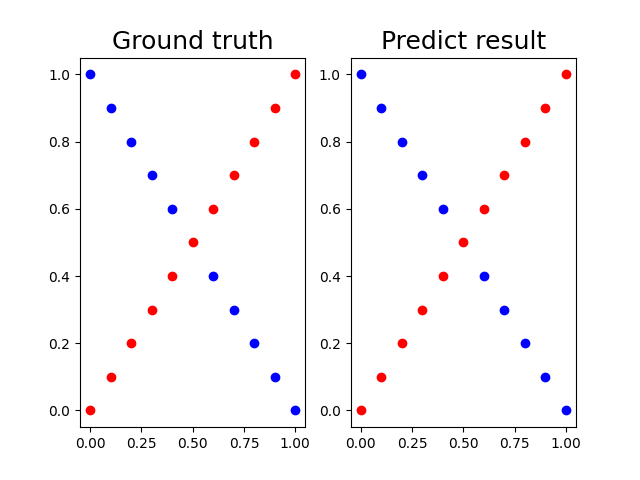
\includegraphics{figures/results/xor_lr1_n32_e500}
\end{tabular}%
}
\caption{\textbf{Decision boundaries for XOR classification with varying numbers of neurons.} From top-left to bottom-right: n=4, n=8, n=16, and n=32. The XOR problem requires sufficient network capacity to form proper non-linear decision boundaries, with networks having fewer than 16 neurons failing to capture the underlying pattern.}
\label{fig:res_xor_n}
\end{figure}

\begin{table}[t]
\centering
\caption{\textbf{Classification accuracy (\%) with different numbers of neurons on linear and XOR datasets.} While the linear problem can be solved with as few as 4 neurons, the XOR problem requires at least 16 neurons to achieve optimal performance.}
\label{tab:num}
\begin{tabular}{@{}ccc@{}}
\toprule
\textbf{Number of Neurons} & \textbf{Linear} & \textbf{XOR} \\ \midrule
4          & 100.0            & 52.4         \\
8           & 99.0           & 52.4        \\
16         & 99.0            & 100.0         \\
32        & 100.0            & 100.0         \\ \bottomrule
\end{tabular}
\end{table}

\subsection{Analysis on Activation Functions}
In our default configuration, we use a ReLU activation in the first layer and a Sigmoid activation in the second layer. In this analysis, we investigate the impact of removing the activation function in the first layer while retaining the Sigmoid activation in the second layer.

The presence of non-linear activation functions is a critical component in neural networks, particularly for solving complex problems that are not linearly separable. Our experiments demonstrate this fundamental principle by comparing the performance of networks with and without a ReLU activation in the first layer.

For the linear classification task, both configurations achieve comparable performance (99.0\% accuracy in both cases). This outcome is expected since linear problems can be solved with linear transformations alone. The addition of a non-linear activation function provides minimal benefit for such problems, as demonstrated by the nearly identical loss curves and decision boundaries in Figures \ref{fig:loss_linear_act} and \ref{fig:res_linear_act}.

However, for the XOR problem, which is inherently non-linearly separable, the absence of a non-linear activation function in the first layer dramatically reduces performance from 100.0\% to 71.4\% accuracy, as shown in Table \ref{tab:act}. This result underscores the theoretical limitation that a network without non-linear transformations is functionally equivalent to a single linear layer, regardless of its depth. The XOR problem, which requires forming complex decision boundaries that separate data points diagonally, cannot be solved effectively by such linear combinations.

Figures \ref{fig:loss_xor_act} and \ref{fig:res_xor_act} illustrate this stark contrast visually. With the ReLU activation, the network successfully learns the characteristic non-linear decision boundary needed for XOR classification. Without the ReLU, the network attempts to approximate the solution with a linear boundary, resulting in performance only marginally better than random guessing.

This experiment empirically validates the universal approximation theorem, which states that neural networks with at least one hidden layer and non-linear activation functions can approximate any continuous function. When we remove this non-linearity, the network loses its ability to model complex relationships in the data.

\begin{figure}[H]
\resizebox{0.95\linewidth}{!}{%
\begin{tabular}{cc}
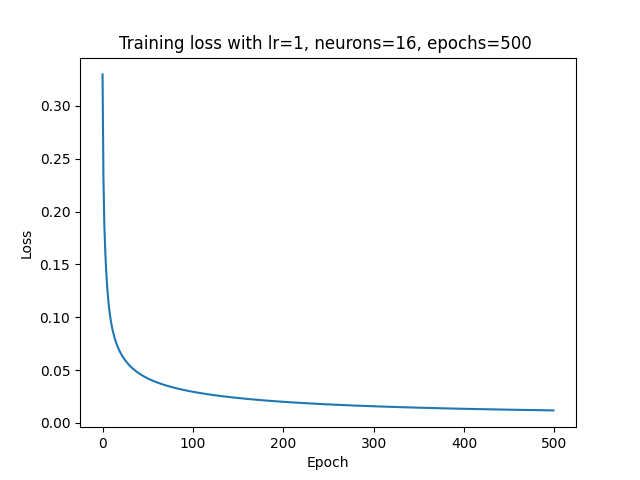
\includegraphics{figures/results/loss_linear_lr1_n16_e500} & 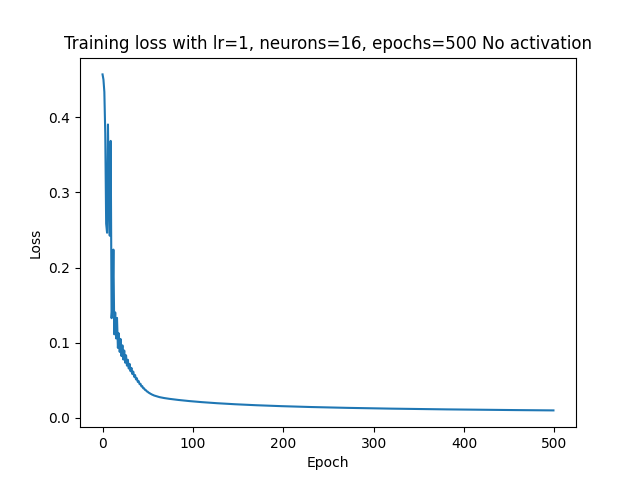
\includegraphics{figures/results/loss_linear_lr1_n16_e500_no_acti}
\end{tabular}%
}
\caption{\textbf{Loss trajectories for linear classification with different activation functions.} Left: ReLU in first layer, Sigmoid in second layer. Right: No activation in first layer, Sigmoid in second layer. Both configurations converge effectively for the linear problem, showing minimal difference in convergence behavior.}
\label{fig:loss_linear_act}
\end{figure}

\begin{figure}[H]
\resizebox{0.95\linewidth}{!}{%
\begin{tabular}{cc}
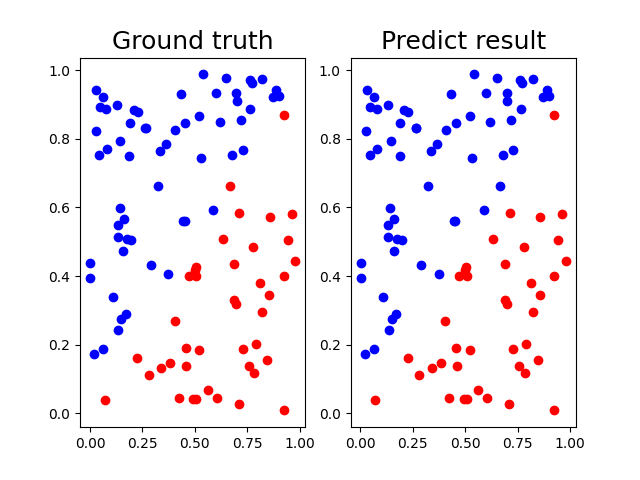
\includegraphics{figures/results/linear_lr1_n16_e500} & 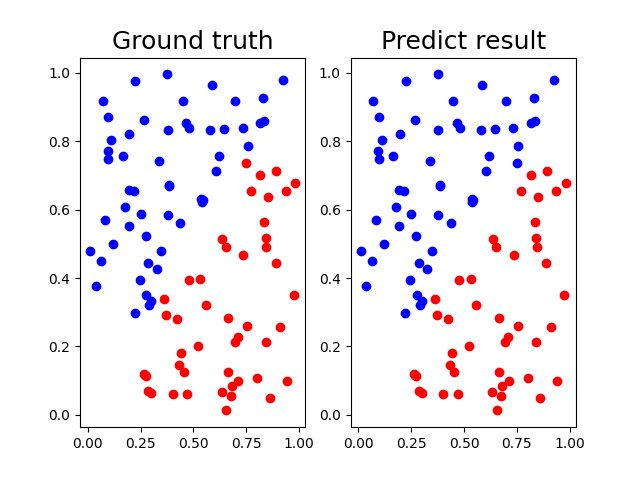
\includegraphics{figures/results/linear_lr1_n16_e500_no_acti}
\end{tabular}%
}
\caption{\textbf{Decision boundaries for linear classification with different activation functions.} Left: ReLU in first layer, Sigmoid in second layer. Right: No activation in first layer, Sigmoid in second layer. Both configurations produce similar decision boundaries for the linear problem, demonstrating that non-linearity is not essential for linearly separable tasks.}
\label{fig:res_linear_act}
\end{figure}

\begin{figure}[H]
\resizebox{0.95\linewidth}{!}{%
\begin{tabular}{cc}
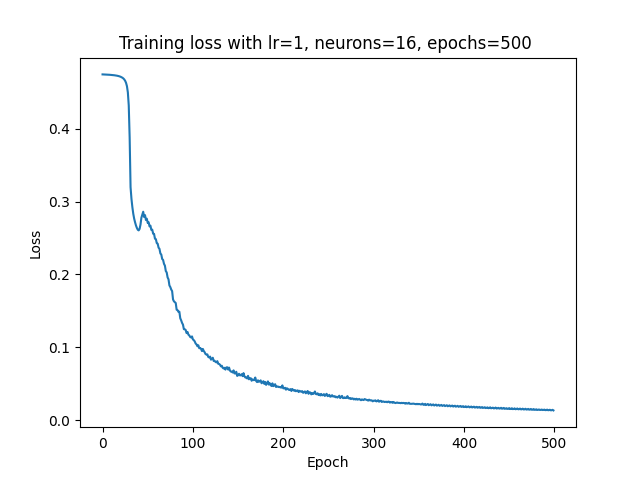
\includegraphics{figures/results/loss_xor_lr1_n16_e500} & 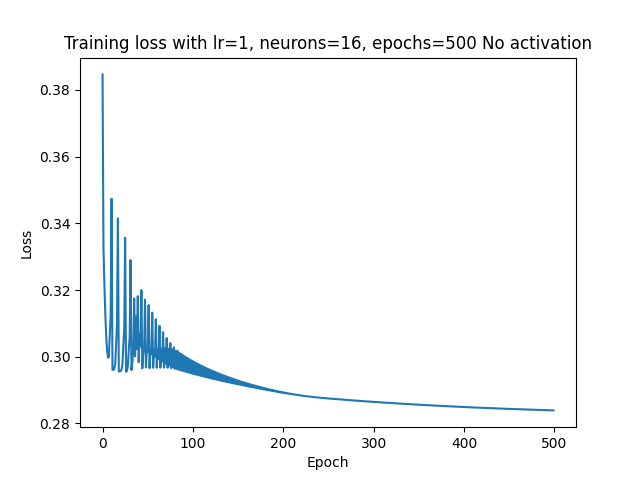
\includegraphics{figures/results/loss_xor_lr1_n16_e500_no_acti}
\end{tabular}%
}
\caption{\textbf{Loss trajectories for XOR classification with different activation functions.} Left: ReLU in first layer, Sigmoid in second layer. Right: No activation in first layer, Sigmoid in second layer. The absence of non-linearity in the first layer significantly impedes convergence for the XOR problem, with the loss unable to reach the same minimum as the network with ReLU activation.}
\label{fig:loss_xor_act}
\end{figure}

\begin{figure}[H]
\resizebox{0.95\linewidth}{!}{%
\begin{tabular}{cc}
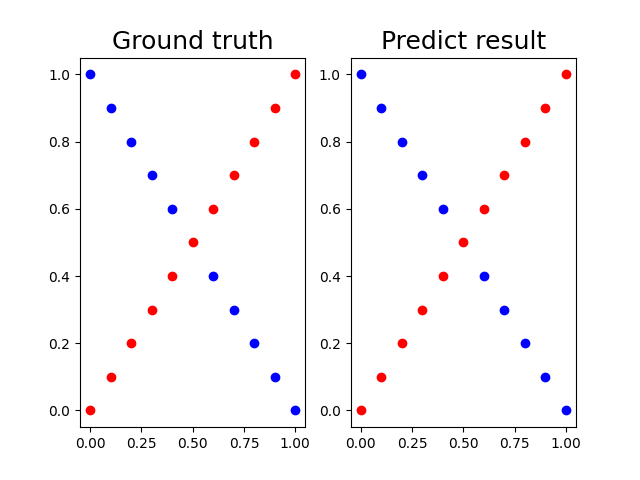
\includegraphics{figures/results/xor_lr1_n16_e500} & 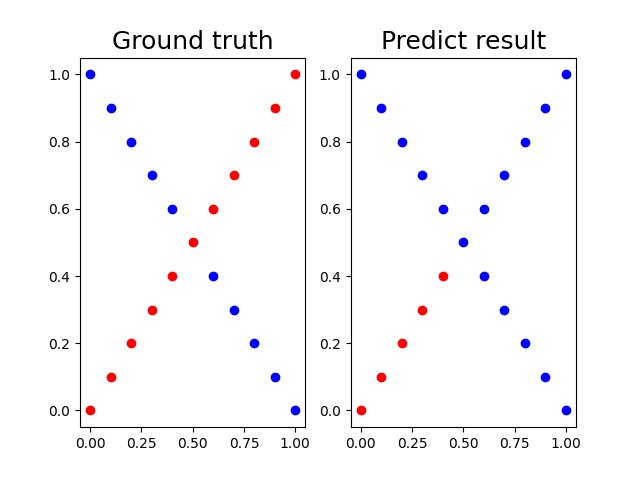
\includegraphics{figures/results/xor_lr1_n16_e500_no_acti}
\end{tabular}%
}
\caption{\textbf{Decision boundaries for XOR classification with different activation functions.} Left: ReLU in first layer, Sigmoid in second layer. Right: No activation in first layer, Sigmoid in second layer. Without a non-linear activation in the first layer, the model fails to learn the proper complex decision boundary required for the XOR problem.}
\label{fig:res_xor_act}
\end{figure}

\begin{table}[t]
\centering
\caption{\textbf{Classification accuracy (\%) with different activation function configurations on linear and XOR datasets.} While the linear problem can be solved effectively with or without ReLU in the first layer, the XOR problem requires non-linearity in the hidden layer to achieve acceptable performance.}
\label{tab:act}
\begin{tabular}{@{}ccc@{}}
\toprule
\textbf{Activation Functions} & \textbf{Linear} & \textbf{XOR} \\ \midrule
ReLU(), Sigmoid()          & 99.0            & 100.0        \\
None, Sigmoid()           & 99.0           & 71.4        \\ \bottomrule	
\end{tabular}
\end{table}

\section{Questions}
\paragraph{What is the purpose of activation functions?}
Activation functions serve several critical purposes in neural networks:

\begin{enumerate}
    \item \textbf{Non-linearity introduction}: The most fundamental role of activation functions is to introduce non-linearity into the network. Without them, no matter how many layers a neural network has, it would be equivalent to a single linear transformation. Non-linearity enables the network to learn complex patterns and approximate arbitrary functions, as demonstrated by the universal approximation theorem.

    \item \textbf{Feature transformation}: Activation functions transform input signals into different representational spaces, enabling the network to learn hierarchical feature representations across layers. Each layer progressively transforms the data into more abstract and task-relevant representations.

    \item \textbf{Output normalization}: Functions like Sigmoid constrain outputs to specific ranges (e.g., [0,1]), which is particularly useful for classification problems where outputs represent probabilities. Similarly, the softmax function normalizes outputs into a probability distribution, making it suitable for multi-class classification.

    \item \textbf{Gradient flow regulation}: Certain activation functions, such as ReLU and its variants, help mitigate the vanishing gradient problem by maintaining stronger gradient signals during backpropagation, particularly in deeper networks.
\end{enumerate}

Our experiments with the XOR problem empirically validate the necessity of non-linear activation functions. When we removed the ReLU activation from the first layer, the network's performance on the XOR problem degraded significantly, demonstrating that non-linearity is essential for solving problems that are not linearly separable.

\paragraph{What might happen if the learning rate is too large or too small?}
The learning rate is a critical hyperparameter that governs the step size during gradient-based optimization. When improperly tuned, several issues can arise:

\textbf{If the learning rate is too large:}
\begin{itemize}
    \item \textbf{Overshoot and divergence}: The optimization algorithm may overshoot the minimum of the loss function, causing parameters to oscillate or diverge completely, as seen in our experiments with learning rate=10.
    \item \textbf{Training instability}: Large oscillations in the loss function make the training process unstable and unpredictable.
    \item \textbf{Exploding gradients}: In extreme cases, weights can grow to infinity, leading to numerical overflow errors.
    \item \textbf{Suboptimal convergence}: Even if convergence occurs, the model may settle in a suboptimal region of the parameter space, resulting in reduced performance.
    \item \textbf{Inability to capture fine details}: Large updates prevent the model from making precise adjustments needed to learn subtle patterns in the data.
\end{itemize}

\textbf{If the learning rate is too small:}
\begin{itemize}
    \item \textbf{Slow convergence}: Training progresses at an exceedingly slow pace, requiring many more iterations to reach acceptable performance, as demonstrated in our experiments with learning rate=0.01.
    \item \textbf{Local minima trapping}: The model may become trapped in local minima or saddle points, unable to escape due to insufficient momentum in parameter updates.
    \item \textbf{Premature convergence}: Early stopping criteria may terminate training before the model reaches optimal performance, giving the false impression of convergence.
    \item \textbf{Underfitting}: Insufficient exploration of the parameter space may lead to underfitting, particularly when training time is constrained.
    \item \textbf{Sensitivity to initialization}: With small updates, the final model performance becomes highly dependent on the initial parameter values.
\end{itemize}

Our experimental results in Table \ref{tab:lr} clearly demonstrate these effects, with both very high (10) and very low (0.01) learning rates yielding significantly reduced performance compared to the optimal rate of 1.0. This highlights the importance of proper learning rate tuning in neural network training.

\paragraph{What is the purpose of weights and biases in a neural network?}
Weights and biases are the fundamental learnable parameters that enable neural networks to adapt to data and solve complex tasks:

\textbf{Weights:}
\begin{itemize}
    \item \textbf{Knowledge representation}: Weights encode the learned relationships and patterns extracted from the training data, forming the "knowledge" of the neural network.
    \item \textbf{Feature importance}: They determine the relative importance of each input feature to neurons in subsequent layers, effectively learning which features are most relevant for the task.
    \item \textbf{Signal modulation}: Weights modulate the strength of connections between neurons, amplifying or attenuating signals as they propagate through the network.
    \item \textbf{Hierarchical feature learning}: Through multiple layers, weights transform raw inputs into increasingly abstract and task-relevant representations, enabling the deep hierarchical feature learning that makes neural networks powerful.
    \item \textbf{Function approximation}: The collective pattern of weights allows neural networks to approximate complex functions, with the universal approximation theorem guaranteeing that sufficiently large networks can approximate any continuous function.
\end{itemize}

\textbf{Biases:}
\begin{itemize}
    \item \textbf{Activation threshold adjustment}: Biases shift the activation function left or right, effectively controlling the threshold at which neurons activate. This allows the network to model data that is not centered around the origin.
    \item \textbf{Default behavior specification}: They determine a neuron's output when all inputs are zero, providing a baseline activation level that can be either excitatory or inhibitory.
    \item \textbf{Representational flexibility}: Biases add an extra degree of freedom to each neuron, significantly increasing the expressive power of the network by allowing it to represent functions that do not pass through the origin.
    \item \textbf{Learning intercepts}: In the context of regression or function approximation, biases allow the network to learn the y-intercept of functions, which would be impossible with weights alone.
    \item \textbf{Class prior incorporation}: In classification tasks, biases can implicitly model the prior probability of different classes, making the network more sensitive to frequent classes and less sensitive to rare ones.
\end{itemize}

Together, weights and biases form the complete parameter set that is optimized during training through backpropagation and gradient descent. Our experimental results demonstrate their effectiveness, particularly in learning complex non-linear decision boundaries for the XOR problem.

\section{Extra} \label{sec:extra}

\subsection{ReLU function}
The Rectified Linear Unit (ReLU) activation function is formally defined as:
\begin{equation}
\text{ReLU}(x) = \max(0, x) \, .
\end{equation}
Its derivative is: 
\begin{equation}
\frac{d}{dx} \text{ReLU}(x) =
\begin{cases}
	1, & \text{if } x > 0 \\
	0, & \text{otherwise.}
\end{cases}
\end{equation}

This piecewise-linear activation function has become one of the most widely used in deep learning due to its computational efficiency and effectiveness in mitigating the vanishing gradient problem.

\begin{code}
\captionof{listing}{\textbf{Implementation of the ReLU activation function.}}
\label{code: relu}
\begin{minted}
class ReLU(NNModule):
    def __init__(self):
        self.input = None

    def forward(self, x):
        self.input = x
        return np.maximum(0, x)

    def backward(self, grad):
        return grad * np.where(self.input > 0, 1, 0)

    def parameters(self):
        return []  # Activation functions don't have trainable parameters
\end{minted}
\end{code}

\end{document}